
\paragraph{}
For this problem we are going to compute dynamically the optimal triangulation of every sub-polygon made of consecutive vertices (see Fig.\ref{fig:Diagramme1} for an example).

\begin{figure}[h]
	\centering
		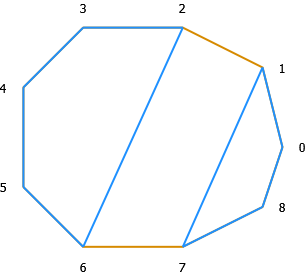
\includegraphics[width=0.5\textwidth]{Diagramme1.png}
	\caption{Two examples of sub-polygon for which we compute optimal triangulation}
	\label{fig:Diagramme1}
\end{figure}

\paragraph{}
We can easily keep in a $n\times n$ matrix the values of these triangulations : In cell $i,j$ we keep the value of the best triangulation of the sub-polygon built with the $j$ vertices $i,i+1,...,i+j-1$.

\paragraph{} 
We compute the optimal triangulation row after row, increasing the size of the sub-polygon. At first we see that sub-polygons of size three are triangles and have triangulations of value 0. Then, when faced to a new sub-polygon $(i,j)$, we look at every triangle we can build with the edge $(i, i+j-1)$. For each of these triangles we compute the value of the best triangulation that includes it and we memorize the best of all (see Fig. \ref{fig:Diagramme2}). This computations are easy considering we already computed all the smaller consecutive sub-polygons. Each of these steps takes $O(n)$ time.

\begin{figure}[h]
	\centering
		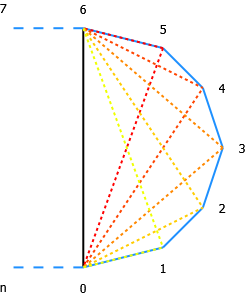
\includegraphics[width=0.5\textwidth]{Diagramme2.png}
	\caption{For $heptagon(0123456)$, the best triangulation that includes $triangle(026)$ has value $length(02) + length(26) + triangulation(23456) + triangulation(012)$}
	\label{fig:Diagramme2}
\end{figure}

\paragraph{}
The overall complexity is $O(n^3)$ in time and $O(n^2)$ in space. To retrieve the optimal triangulation we just need to remember from where were taken the minimums and follow the way back to the first row.

